\documentclass[10pt]{article}

\usepackage[a4paper,margin=0.65in]{geometry}
\usepackage{amsmath,amssymb}
\usepackage{graphicx}
\usepackage{booktabs}
\usepackage{array}
\usepackage{float}
\usepackage{hyperref}
\usepackage{enumitem}
\usepackage{xcolor}
\usepackage{tikz}
\usetikzlibrary{positioning,arrows.meta,shapes.geometric,fit,calc}

\setlist{nosep,leftmargin=*}
\renewcommand{\arraystretch}{1.2}
\setlength{\parindent}{0pt}
\setlength{\parskip}{2pt}

\tikzset{
layer/.style={
draw,
rounded corners,
minimum width=1.7cm,
minimum height=0.65cm,
align=center,
fill=blue!10,
font=\scriptsize
},
smalllayer/.style={
draw,
rounded corners,
minimum width=1.35cm,
minimum height=0.58cm,
align=center,
fill=green!10,
font=\scriptsize
},
arrow/.style={
-{Latex[length=2mm]},
thin
}
}

\begin{document}

%%%%%%%%%%%%%%%%%%%%%%%%%%%%%%%%%%%%%%%%%%%%%%%%%%%%%%%%%%%%
% TITLE
%%%%%%%%%%%%%%%%%%%%%%%%%%%%%%%%%%%%%%%%%%%%%%%%%%%%%%%%%%%%

\begin{center}

{\large\textbf{Shiv Nadar University Chennai}}

\vspace{2mm}

{\normalsize\textbf{CS3807 -- Deep Learning Laboratory}}

\vspace{2mm}

{\large\textbf{Experiment 6}}

\vspace{1mm}

{\normalsize\textbf{End-to-End Study of RNN, LSTM and GRU for}}

{\normalsize\textbf{Sequence Learning and Video Understanding}}

\end{center}

\vspace{3mm}

\begin{tabular}{|p{3.4cm}|p{9.0cm}|p{1.4cm}|}
\hline
Degree \& Branch &
B.Tech Artificial Intelligence \& Data Science &
Semester V\\
\hline
Subject Code \& Name &
CS3807 -- Deep Learning Laboratory &
AY: 2026--27\\
\hline
\end{tabular}

%%%%%%%%%%%%%%%%%%%%%%%%%%%%%%%%%%%%%%%%%%%%%%%%%%%%%%%%%%%%
\section*{1. Objective}

The objective of this experiment is to develop an end-to-end understanding of
recurrent sequence learning by implementing and comparing Vanilla RNN, LSTM
and GRU models. The experiment also introduces Backpropagation Through Time
(BPTT), the limitations of conventional RNNs, and the use of CNN-extracted
features with recurrent networks for video understanding.

The experiment uses the UCI Human Activity Recognition Using Smartphones
dataset as the primary sequence dataset. Temporal input sequences were
prepared and visualized, RNN/LSTM/GRU models were trained, their performance,
convergence and generalization were analyzed, and the pipeline was extended
to video understanding using CNN feature extraction followed by an LSTM or
GRU. A small synthetic sequence-to-sequence task was included at the end to
demonstrate the encoder--decoder framework.

%%%%%%%%%%%%%%%%%%%%%%%%%%%%%%%%%%%%%%%%%%%%%%%%%%%%%%%%%%%%
\section*{2. Learning Outcomes}

After completing this experiment, the following outcomes were achieved:

\begin{itemize}
\item representing sequential data using the $(N,T,F)$ input format;
\item explaining the architecture and operation of a Vanilla RNN;
\item explaining Backpropagation Through Time and the vanishing/exploding gradient challenges;
\item implementing sequence classification using SimpleRNN, LSTM and GRU;
\item comparing RNN, LSTM and GRU using quantitative performance measures;
\item interpreting training/validation curves and confusion matrices;
\item explaining the role of CNNs in extracting spatial features from video frames;
\item constructing a CNN--LSTM or CNN--GRU pipeline for video understanding;
\item explaining the encoder--decoder architecture for sequence-to-sequence learning; and
\item drawing conclusions using predictive performance, model complexity and computational cost.
\end{itemize}

%%%%%%%%%%%%%%%%%%%%%%%%%%%%%%%%%%%%%%%%%%%%%%%%%%%%%%%%%%%%
\section*{3. Dataset and Experimental Setup}

\textbf{Primary Dataset: UCI Human Activity Recognition Using Smartphones}

The UCI Human Activity Recognition (HAR) dataset contains smartphone sensor
measurements collected from subjects performing six activities:

\begin{itemize}
\item WALKING
\item WALKING UPSTAIRS
\item WALKING DOWNSTAIRS
\item SITTING
\item STANDING
\item LAYING
\end{itemize}

The raw inertial signal files were used rather than the already-computed
561-feature vectors. Each activity window contains 128 temporal measurements.
The three-axis body acceleration, three-axis gyroscope and three-axis total
acceleration signals provide nine channels, giving the input representation

\[
X\in\mathbb{R}^{N\times128\times9}.
\]

Dataset source:
\url{https://archive.ics.uci.edu/dataset/240/human+activity+recognition+using+smartphones}

\textbf{Laboratory subset used:} A balanced subset of 3{,}000 windows (500
per class) was drawn from the official UCI training partition
(7{,}352 windows) using a fixed random seed (42), to keep the many
comparison runs practical while preserving all six classes in equal
proportion.

\textbf{Important:} The same train/validation/test protocol and
preprocessing was used for RNN, LSTM and GRU so that the comparison is
controlled.

\subsection*{Expected Input}

For one sample:

\[
X_i\in\mathbb{R}^{128\times9}.
\]

For a batch of 32 samples:

\[
X_{\mathrm{batch}}\in\mathbb{R}^{32\times128\times9}.
\]

The dimensions represent:

\begin{center}
\begin{tabular}{|c|c|l|}
\hline
Dimension & Meaning & Observed value\\
\hline
$N$ & Number of sequences & 3{,}000 (2{,}100/450/450 train/val/test)\\
$T$ & Time steps per sequence & 128\\
$F$ & Features/channels per time step & 9\\
\hline
\end{tabular}
\end{center}

Therefore, the model receives a three-dimensional tensor rather than a
conventional two-dimensional tabular matrix.

%%%%%%%%%%%%%%%%%%%%%%%%%%%%%%%%%%%%%%%%%%%%%%%%%%%%%%%%%%%%
\section*{4. Overall Experimental Pipeline}

The complete sequence-classification pipeline is:

\begin{center}
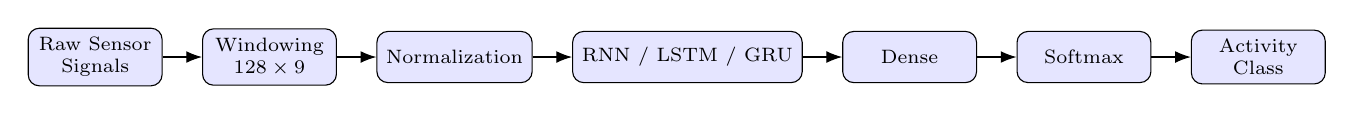
\begin{tikzpicture}[node distance=5mm]
\node[layer](a){Raw Sensor\\Signals};
\node[layer,right=of a](b){Windowing\\$128\times9$};
\node[layer,right=of b](c){Normalization};
\node[layer,right=of c](d){RNN / LSTM / GRU};
\node[layer,right=of d](e){Dense};
\node[layer,right=of e](f){Softmax};
\node[layer,right=of f](g){Activity\\Class};

\foreach \x/\y in {a/b,b/c,c/d,d/e,e/f,f/g}
\draw[arrow](\x)--(\y);
\end{tikzpicture}
\end{center}

The three recurrent models used the same input, output layer, optimizer,
batch size and evaluation protocol.

%%%%%%%%%%%%%%%%%%%%%%%%%%%%%%%%%%%%%%%%%%%%%%%%%%%%%%%%%%%%
\section*{5. Preprocessing}

The following preprocessing steps were performed:

\begin{enumerate}
\item Load the raw inertial signals.
\item Arrange every observation window as $128\times9$.
\item Assign one activity label to each window.
\item Encode the six activity labels (0--5).
\item Normalize the input using per-channel z-score statistics calculated
from the training split only.
\item Create stratified training, validation and test sets (70/15/15).
\item Verify the class distribution.
\end{enumerate}

The test data was not used during model selection or hyperparameter tuning.

\subsection*{Observed Preprocessing Output}

\begin{verbatim}
Input tensor shape:
Training   : (2100, 128, 9)
Validation : (450, 128, 9)
Testing    : (450, 128, 9)

Number of classes: 6
Number of features per time step: 9
Sequence length: 128
\end{verbatim}

\begin{center}
\begin{tabular}{|l|c|c|c|}
\hline
Class & Train & Validation & Test\\
\hline
WALKING & 350 & 75 & 75\\
WALKING UPSTAIRS & 350 & 75 & 75\\
WALKING DOWNSTAIRS & 350 & 75 & 75\\
SITTING & 350 & 75 & 75\\
STANDING & 350 & 75 & 75\\
LAYING & 350 & 75 & 75\\
\hline
TOTAL & 2{,}100 & 450 & 450\\
\hline
\end{tabular}
\end{center}

Each class is exactly balanced across all three splits by construction. After
normalization, the per-channel training-set mean was approximately 0 and the
per-channel training-set standard deviation was approximately 1 for all nine
channels, confirming the z-score normalization was applied correctly.

%%%%%%%%%%%%%%%%%%%%%%%%%%%%%%%%%%%%%%%%%%%%%%%%%%%%%%%%%%%%
\section*{6. Temporal Data Visualization}

\textbf{Plot 1: Sensor signal versus time}

One representative window from each of the six activity classes is plotted
for three channels (\texttt{body\_acc\_x}, \texttt{body\_gyro\_x},
\texttt{total\_acc\_x}), separated into dynamic activities (WALKING, WALKING
UPSTAIRS, WALKING DOWNSTAIRS) and static activities (SITTING, STANDING,
LAYING).

\begin{figure}[H]
\centering
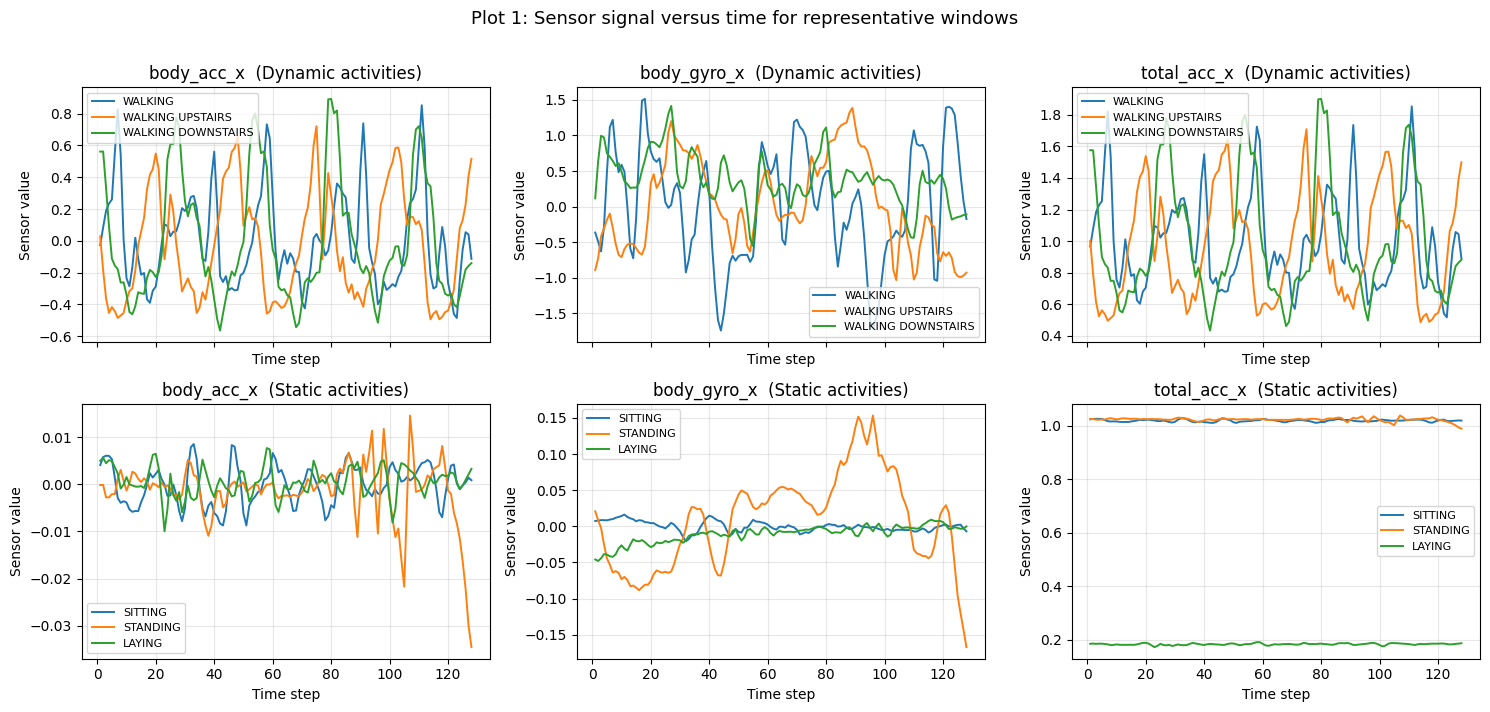
\includegraphics[width=0.95\textwidth]{images/plot1_temporal_sensor_signals.png}
\caption{Plot 1: Sensor signal versus time for representative windows}
\end{figure}

\begin{center}
\begin{tabular}{|l|c|c|c|}
\hline
Activity & body\_acc\_x std & body\_gyro\_x std & total\_acc\_x std\\
\hline
WALKING & 0.2897 & 0.7701 & 0.2893\\
WALKING UPSTAIRS & 0.3352 & 0.6289 & 0.3353\\
WALKING DOWNSTAIRS & 0.3816 & 0.3509 & 0.3806\\
SITTING & 0.0041 & 0.0069 & 0.0041\\
STANDING & 0.0066 & 0.0653 & 0.0067\\
LAYING & 0.0030 & 0.0120 & 0.0030\\
\hline
\end{tabular}
\end{center}

\textbf{Inference:}

\begin{enumerate}
\item \textbf{What temporal pattern is visible?} The three dynamic
activities show large, quasi-periodic oscillations across all 128 time
steps (e.g.\ \texttt{body\_gyro\_x} standard deviation of 0.35--0.77), while
the three static activities are nearly flat with standard deviations roughly
two orders of magnitude smaller (0.003--0.012 for \texttt{body\_acc\_x}).
\item \textbf{Which activities exhibit similar patterns?} WALKING UPSTAIRS
and WALKING DOWNSTAIRS show visually similar oscillation shape and
amplitude to plain WALKING in \texttt{body\_acc\_x} and
\texttt{total\_acc\_x}, which is consistent with the frequent
WALKING~$\leftrightarrow$~WALKING UPSTAIRS confusions observed later in the
RNN confusion matrix (Section 15). Among the static activities, SITTING and
STANDING have comparably small but non-zero \texttt{body\_gyro\_x}
variation (0.0069 and 0.0653 respectively), whereas LAYING is the flattest
of all six.
\item \textbf{Why is the ordering of measurements important?} The activity
label depends on the temporal shape of the signal (the oscillation
frequency and phase relationships across channels), not on the set of
sampled values alone; shuffling the 128 time steps within a window would
destroy this structure even though the marginal distribution of sensor
values would be unchanged, which is exactly why a model that respects
sequence order (RNN/LSTM/GRU) is required rather than a time-step-agnostic
classifier.
\end{enumerate}

%%%%%%%%%%%%%%%%%%%%%%%%%%%%%%%%%%%%%%%%%%%%%%%%%%%%%%%%%%%%
\section*{7. Vanilla RNN Architecture}

A Vanilla RNN maintains a hidden state that is updated at every time step:

\[
h_t=\tanh(W_xx_t+W_hh_{t-1}+b_h).
\]

The output can be written as

\[
y_t=g(W_yh_t+b_y).
\]

For sequence classification, the final hidden representation is passed to a
classifier.

\begin{center}
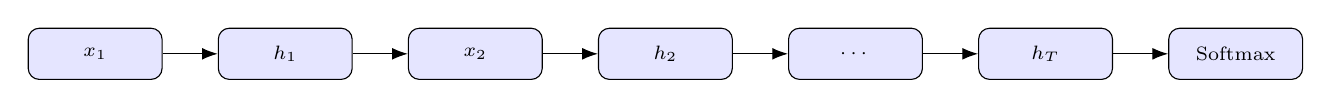
\begin{tikzpicture}[node distance=7mm]
\node[layer](x1){$x_1$};
\node[layer,right=of x1](h1){$h_1$};
\node[layer,right=of h1](x2){$x_2$};
\node[layer,right=of x2](h2){$h_2$};
\node[layer,right=of h2](x3){$\cdots$};
\node[layer,right=of x3](h3){$h_T$};
\node[layer,right=of h3](y){Softmax};

\draw[arrow](x1)--(h1);
\draw[arrow](h1)--(x2);
\draw[arrow](x2)--(h2);
\draw[arrow](h2)--(x3);
\draw[arrow](x3)--(h3);
\draw[arrow](h3)--(y);
\end{tikzpicture}
\end{center}

The diagram represents the unrolled view of an RNN. The same recurrent
weights are reused across time steps. The hidden state $h_t$ represents a
compressed summary of everything the network has seen in the sequence up to
time $t$, updated recursively rather than recomputed from scratch at every
step.

%%%%%%%%%%%%%%%%%%%%%%%%%%%%%%%%%%%%%%%%%%%%%%%%%%%%%%%%%%%%
\section*{8. Backpropagation Through Time}

When an RNN is unrolled, the loss depends on the sequence of hidden states.
Backpropagation Through Time (BPTT) propagates the error backward through
the recurrent steps.

\begin{center}
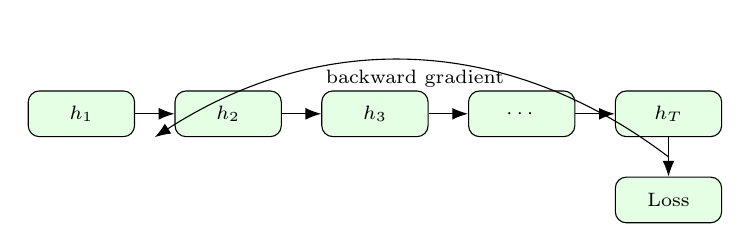
\begin{tikzpicture}[node distance=5mm]
\node[smalllayer](a){$h_1$};
\node[smalllayer,right=of a](b){$h_2$};
\node[smalllayer,right=of b](c){$h_3$};
\node[smalllayer,right=of c](d){$\cdots$};
\node[smalllayer,right=of d](e){$h_T$};
\node[smalllayer,below=of e](l){Loss};

\draw[arrow](a)--(b);
\draw[arrow](b)--(c);
\draw[arrow](c)--(d);
\draw[arrow](d)--(e);
\draw[arrow](e)--(l);

\draw[arrow]($(e.south)!0.5!(l.north)$) to[bend right=35]
node[below,font=\scriptsize]{backward gradient} ($(a.south)!0.5!(b.south)$);
\end{tikzpicture}
\end{center}

Repeated multiplication of derivatives through many time steps can cause
gradients to become extremely small or extremely large.

\subsection*{Challenges}

\begin{itemize}
\item Vanishing gradients
\item Exploding gradients
\item Difficulty learning long-term dependencies
\item Sequential computation and limited parallelism
\end{itemize}

The vanishing-gradient problem can be conceptually represented as

\[
\left|\frac{\partial h_t}{\partial h_{t-k}}\right|\rightarrow0
\]

while exploding gradients correspond to very large gradient magnitudes. Both
arise because $\partial h_t/\partial h_{t-k}$ is a product of $k$ Jacobian
terms (each involving $W_h$ and the derivative of $\tanh$); if the dominant
eigenvalue of this repeated product is consistently below 1 the product
shrinks geometrically toward zero, and if it is consistently above 1 the
product grows geometrically.

\subsection*{Numerical Exercise}

Consider

\[
x_1=0.5,\qquad x_2=0.7,\qquad x_3=0.2,
\]

\[
h_0=0,\qquad W_x=0.5,\qquad W_h=0.8,\qquad b=0.1.
\]

Using $h_t=\tanh(W_xx_t+W_hh_{t-1}+b)$:

\begin{center}
\begin{tabular}{|c|l|c|c|}
\hline
State & Pre-activation expression & Pre-activation & $h_t=\tanh(\cdot)$\\
\hline
$h_1$ & $0.5(0.5)+0.8(0)+0.1$ & 0.350000 & 0.336376\\
$h_2$ & $0.5(0.7)+0.8(0.336376)+0.1$ & 0.719100 & 0.616352\\
$h_3$ & $0.5(0.2)+0.8(0.616352)+0.1$ & 0.693081 & 0.599958\\
\hline
\end{tabular}
\end{center}

A Keras \texttt{SimpleRNN} layer with its weights manually set to
$W_x=0.5$, $W_h=0.8$, $b=0.1$ was run on the same input sequence and produced
$h_1,h_2,h_3 = 0.336376,\ 0.616352,\ 0.599958$, matching the manual/NumPy
computation to a maximum absolute difference of $5.9\times10^{-8}$ (floating
point precision only), confirming the hand calculation is correct.

%%%%%%%%%%%%%%%%%%%%%%%%%%%%%%%%%%%%%%%%%%%%%%%%%%%%%%%%%%%%
\section*{9. RNN Implementation}

\begin{center}
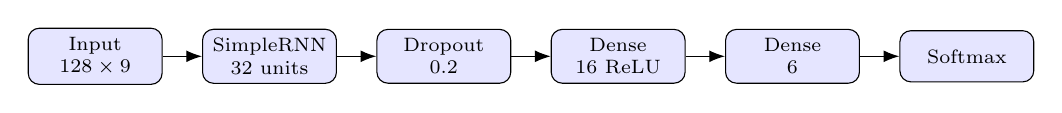
\begin{tikzpicture}[node distance=5mm]
\node[layer](a){Input\\$128\times9$};
\node[layer,right=of a](b){SimpleRNN\\32 units};
\node[layer,right=of b](c){Dropout\\0.2};
\node[layer,right=of c](d){Dense\\16 ReLU};
\node[layer,right=of d](e){Dense\\6};
\node[layer,right=of e](f){Softmax};

\foreach \x/\y in {a/b,b/c,c/d,d/e,e/f}
\draw[arrow](\x)--(\y);
\end{tikzpicture}
\end{center}

\textbf{Training configuration used:}

\begin{center}
\begin{tabular}{|l|l|}
\hline
Parameter & Value\\
\hline
Recurrent units & 32\\
Dropout & 0.2\\
Optimizer & Adam\\
Learning rate & $10^{-3}$\\
Batch size & 32\\
Epochs & 30\\
Loss & Sparse categorical cross-entropy\\
Trainable parameters & 1{,}974\\
\hline
\end{tabular}
\end{center}

The analytical parameter count $u(F+u+1)+\text{head}=32(9+32+1)+658=1{,}974$
matched the Keras-reported trainable parameter count exactly, confirming the
architecture was implemented as specified.

%%%%%%%%%%%%%%%%%%%%%%%%%%%%%%%%%%%%%%%%%%%%%%%%%%%%%%%%%%%%
\section*{10. LSTM Architecture}

LSTM introduces a memory cell and gates to control information flow.

The forget gate is
\[
f_t=\sigma(W_f[h_{t-1},x_t]+b_f),
\]
the input gate is
\[
i_t=\sigma(W_i[h_{t-1},x_t]+b_i),
\]
and the output gate is
\[
o_t=\sigma(W_o[h_{t-1},x_t]+b_o).
\]
The candidate cell state is
\[
\tilde{C}_t=
\tanh(W_C[h_{t-1},x_t]+b_C),
\]
and the cell state is
\[
C_t=f_tC_{t-1}+i_t\tilde{C}_t.
\]
The hidden state is
\[
h_t=o_t\tanh(C_t).
\]

\begin{center}
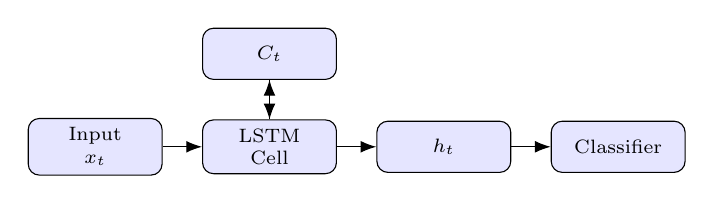
\begin{tikzpicture}[node distance=5mm]
\node[layer](a){Input\\$x_t$};
\node[layer,right=of a](b){LSTM\\Cell};
\node[layer,right=of b](c){$h_t$};
\node[layer,above=of b](d){$C_t$};
\node[layer,right=of c](e){Classifier};

\draw[arrow](a)--(b);
\draw[arrow](b)--(c);
\draw[arrow](b)--(d);
\draw[arrow](c)--(e);
\draw[arrow](d)--(b);
\end{tikzpicture}
\end{center}

\textbf{Inference:} The cell state $C_t$ acts as a protected memory highway
that is updated by element-wise (additive) interactions rather than being
recomputed by a matrix multiplication and nonlinearity at every step, as in
a Vanilla RNN. The forget gate $f_t$ lets the network discard information no
longer needed, the input gate $i_t$ controls how much of the new candidate
$\tilde{C}_t$ is written in, and the output gate $o_t$ controls how much of
the cell state is exposed as the hidden state. Because the forget-gate path
is (near-)additive rather than repeatedly multiplicative, gradients can flow
backward through many time steps largely unattenuated, directly mitigating
the vanishing-gradient problem of Section 8. This is consistent with LSTM's
substantially higher measured test macro-F1 (94.41\%) than the Vanilla RNN
(76.93\%) in this experiment (Section 14).

%%%%%%%%%%%%%%%%%%%%%%%%%%%%%%%%%%%%%%%%%%%%%%%%%%%%%%%%%%%%
\section*{11. GRU Architecture}

GRU uses two principal gates:
\[
z_t=\sigma(W_z[h_{t-1},x_t]+b_z)
\]
and
\[
r_t=\sigma(W_r[h_{t-1},x_t]+b_r).
\]
The candidate hidden state is
\[
\tilde{h}_t=
\tanh(W_h[r_t\odot h_{t-1},x_t]+b_h).
\]
The hidden state is updated using
\[
h_t=(1-z_t)h_{t-1}+z_t\tilde{h}_t.
\]

\begin{center}
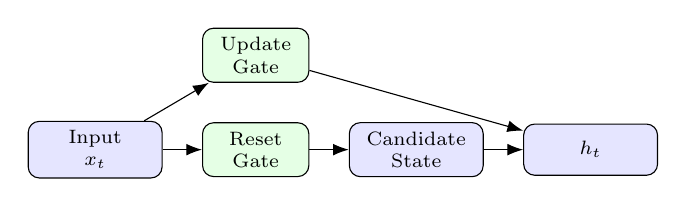
\begin{tikzpicture}[node distance=5mm]
\node[layer](a){Input\\$x_t$};
\node[smalllayer,right=of a](b){Reset\\Gate};
\node[smalllayer,above=of b](c){Update\\Gate};
\node[layer,right=of b](d){Candidate\\State};
\node[layer,right=of d](e){$h_t$};

\draw[arrow](a)--(b);
\draw[arrow](a)--(c);
\draw[arrow](b)--(d);
\draw[arrow](c)--(e);
\draw[arrow](d)--(e);
\end{tikzpicture}
\end{center}

GRU merges the forget and input gates of LSTM into a single update gate
$z_t$, and has no separate cell state: the hidden state $h_t$ itself serves
both roles. This gives GRU fewer parameters than LSTM for the same hidden
size (4{,}758 vs 6{,}006 trainable parameters in this experiment, Section
14), while retaining a gating mechanism that -- like LSTM -- avoids the
Vanilla RNN's purely multiplicative hidden-state update.

%%%%%%%%%%%%%%%%%%%%%%%%%%%%%%%%%%%%%%%%%%%%%%%%%%%%%%%%%%%%
\section*{12. LSTM and GRU Implementation}

The same classifier used for the RNN was reused, replacing only the
recurrent layer; all other experimental conditions (dropout, dense head,
optimizer, learning rate, batch size, epochs, loss, random seed) were held
fixed across the three models so that the comparison is controlled.

\begin{center}
\begin{tabular}{|l|c|c|c|c|}
\hline
Model & Recurrent Layer & Units & Output Classes & Trainable Parameters\\
\hline
RNN & SimpleRNN & 32 & 6 & 1{,}974\\
LSTM & LSTM & 32 & 6 & 6{,}006\\
GRU & GRU & 32 & 6 & 4{,}758\\
\hline
\end{tabular}
\end{center}

%%%%%%%%%%%%%%%%%%%%%%%%%%%%%%%%%%%%%%%%%%%%%%%%%%%%%%%%%%%%
\section*{13. Training Curves (Plots 2 and 3)}

For each of RNN, LSTM and GRU, training/validation loss (Plot 2) and
training/validation accuracy (Plot 3) were generated as a single combined
two-panel figure per model.

\begin{figure}[H]
\centering
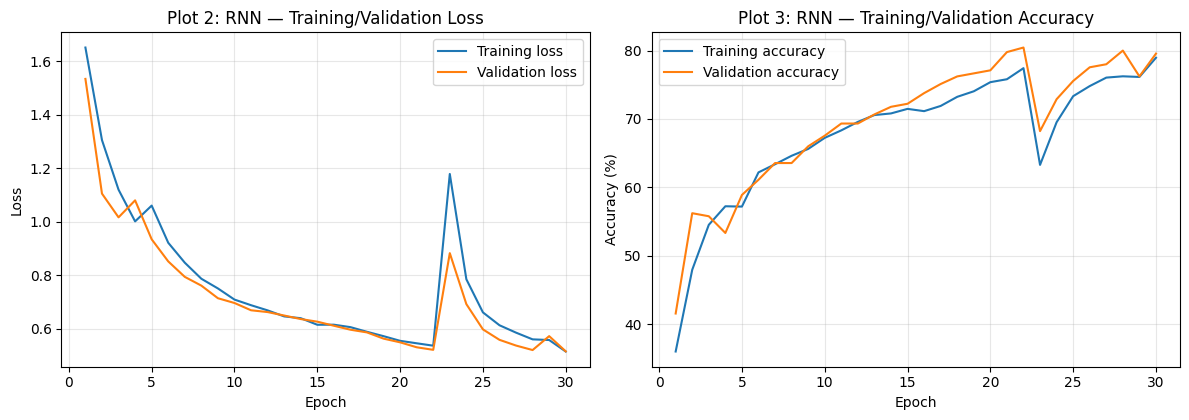
\includegraphics[width=0.92\textwidth]{images/plot23_rnn_loss_accuracy.png}
\caption{Plots 2--3: RNN -- Training/Validation Loss and Accuracy}
\end{figure}

\begin{figure}[H]
\centering
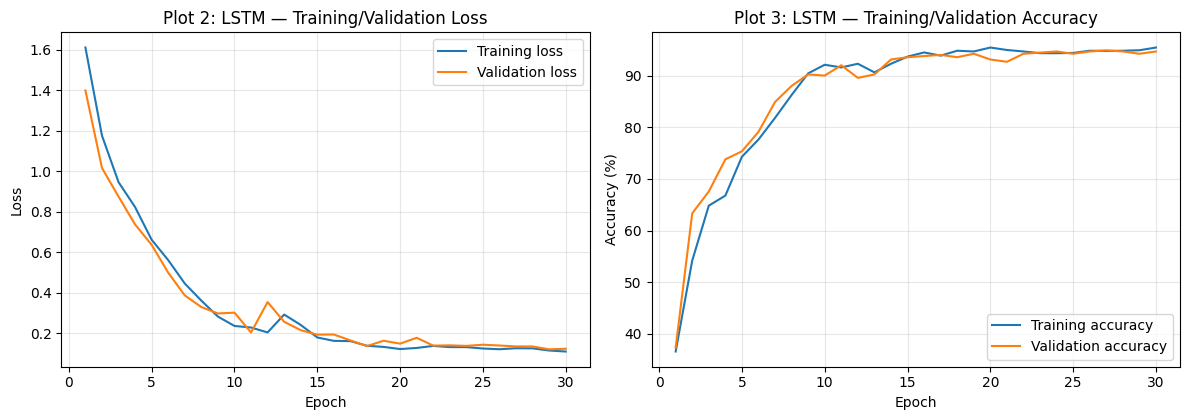
\includegraphics[width=0.92\textwidth]{images/plot23_lstm_loss_accuracy.png}
\caption{Plots 2--3: LSTM -- Training/Validation Loss and Accuracy}
\end{figure}

\begin{figure}[H]
\centering
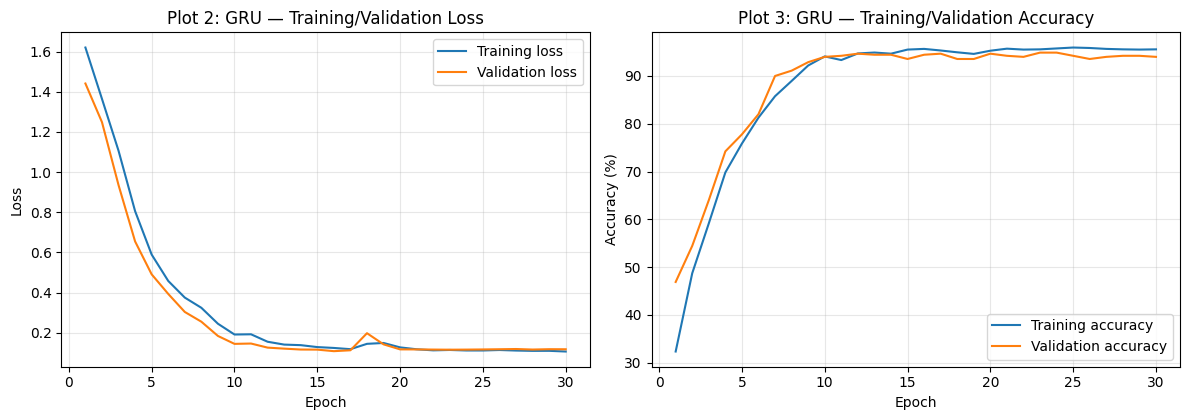
\includegraphics[width=0.92\textwidth]{images/plot23_gru_loss_accuracy.png}
\caption{Plots 2--3: GRU -- Training/Validation Loss and Accuracy}
\end{figure}

\begin{center}
\begin{tabular}{|l|c|c|c|}
\hline
Diagnostic & RNN & LSTM & GRU\\
\hline
Final train loss & 0.5149 & 0.1110 & 0.1064\\
Final val. loss & 0.5156 & 0.1247 & 0.1176\\
Min. val. loss (epoch) & 0.5156 (30) & 0.1220 (29) & 0.1081 (16)\\
Final train acc. & 78.95\% & 95.43\% & 95.57\%\\
Final val. acc. & 79.56\% & 94.67\% & 94.00\%\\
Best val. acc. (epoch) & 80.44\% (22) & 94.89\% (27) & 94.89\% (23)\\
First epoch val.\ acc.\ $\geq$ 90\% & never & 9 & 8\\
\hline
\end{tabular}
\end{center}

\textbf{Inference (convergence behaviour of RNN):} The Vanilla RNN converges
slowly and incompletely: training and validation loss both plateau around
0.51--0.52 with no epoch reaching 90\% validation accuracy, and the curve is
visibly noisier (e.g.\ val. accuracy briefly drops from epoch 20 to epoch
25) than LSTM or GRU. The final train/val.\ accuracy gap is slightly
negative ($-0.60$ points, val.\ above train.), indicating no overfitting --
rather, the RNN is underfitting, consistent with the vanishing-gradient
difficulty it has in exploiting the full 128-step temporal context
(Section 8).

\textbf{Inference (convergence behaviour of LSTM):} LSTM converges quickly
and smoothly, crossing 80\% validation accuracy by epoch 7 and 90\% by
epoch 9, then continuing to improve gradually to a final 94.67\% validation
accuracy. The small positive train--val.\ accuracy gap (0.76 points) and
val.\ loss (0.1247) staying close to train loss (0.1110) indicate mild,
not severe, overfitting by epoch 30.

\textbf{Inference (convergence behaviour of GRU):} GRU converges even
faster than LSTM in the earliest epochs (80\% val.\ accuracy by epoch 6, 90\%
by epoch 8) and reaches its minimum validation loss earliest of the three
models (epoch 16), after which validation loss rises slightly (0.1081 to
0.1176) while training loss keeps falling -- a mild overfitting signal
visible as a widening gap (1.57 points final train--val.\ accuracy gap, the
largest of the three models) in the later epochs of Plot 3.

\textbf{Inference (evidence of overfitting/underfitting):} Taken together,
the RNN under-fits (a small negative gap and loss plateauing well above
zero), while LSTM and GRU both show the signature of mild overfitting
(final training accuracy exceeding validation accuracy by under 2 points,
and validation loss having passed its minimum before epoch 30). None of the
three models shows severe overfitting (e.g.\ a widening gap of many
percentage points) within the 30-epoch budget used here.

%%%%%%%%%%%%%%%%%%%%%%%%%%%%%%%%%%%%%%%%%%%%%%%%%%%%%%%%%%%%
\section*{14. Performance Evaluation}

Each model was evaluated once on the untouched 450-window test set.

\begin{center}
\begin{tabular}{|l|c|c|c|}
\hline
Metric & RNN & LSTM & GRU\\
\hline
Accuracy (\%) & 77.33 & 94.44 & 94.67\\
Macro Precision (\%) & 77.53 & 94.80 & 94.72\\
Macro Recall (\%) & 77.33 & 94.44 & 94.67\\
Macro F1 (\%) & 76.93 & 94.41 & 94.66\\
Parameters & 1{,}974 & 6{,}006 & 4{,}758\\
Training Time (s) & 27.94 & 24.49 & 25.71\\
\hline
\end{tabular}
\end{center}

The Keras-reported trainable-parameter counts matched the analytical
formulas exactly for all three models (RNN: 1{,}974, LSTM: 6{,}006, GRU:
4{,}758), confirming correct architecture implementation.

%%%%%%%%%%%%%%%%%%%%%%%%%%%%%%%%%%%%%%%%%%%%%%%%%%%%%%%%%%%%
\section*{15. Confusion Matrix Analysis}

\begin{figure}[H]
\centering
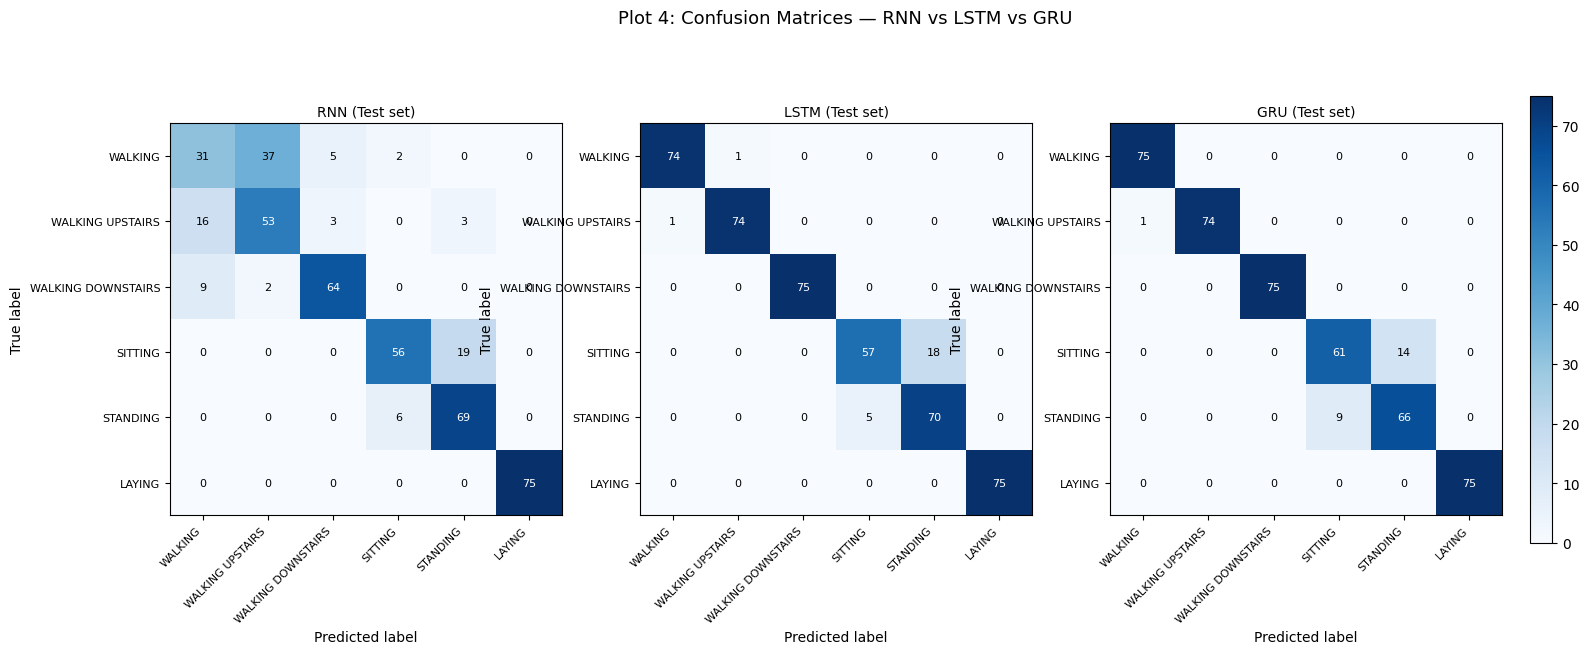
\includegraphics[width=\textwidth]{images/plot4_confusion_all_models.png}
\caption{Plot 4: Confusion Matrices -- RNN vs LSTM vs GRU (Test set)}
\end{figure}

\begin{center}
\begin{tabular}{|l|c|c|c|}
\hline
 & RNN & LSTM & GRU\\
\hline
Highest recall & LAYING (100.00\%) & WALKING DOWNSTAIRS (100.00\%) & WALKING (100.00\%)\\
Lowest recall & WALKING (41.33\%) & SITTING (76.00\%) & SITTING (81.33\%)\\
Most errors (class) & WALKING (44) & SITTING (18) & SITTING (14)\\
Top confusion & WALKING$\rightarrow$WALKING UPSTAIRS (37) & SITTING$\rightarrow$STANDING (18) & SITTING$\rightarrow$STANDING (14)\\
Total misclassified / 450 & 102 & 25 & 24\\
\hline
\end{tabular}
\end{center}

\textbf{Inference (based on the observed matrices):}

\begin{itemize}
\item \textbf{Highest recognition rate:} LAYING is recognized perfectly
(100\% recall) by all three models, and WALKING DOWNSTAIRS is also
perfectly recognized by LSTM. These are the most kinematically distinctive
activities (near-zero motion for LAYING; a strong, asymmetric acceleration
signature for WALKING DOWNSTAIRS).
\item \textbf{Largest number of misclassifications:} For the RNN, WALKING
is by far the most error-prone class (44 of 75 windows misclassified,
mostly as WALKING UPSTAIRS). For both LSTM and GRU, the error profile shifts
entirely to SITTING (18 and 14 misclassified windows respectively).
\item \textbf{Frequently confused pairs:} The RNN confuses the three
dynamic activities among themselves (WALKING$\leftrightarrow$WALKING
UPSTAIRS is its largest single confusion, 37 instances) -- consistent with
the visually similar oscillation patterns observed in Plot 1 (Section 6).
Both LSTM and GRU resolve the dynamic-activity confusions almost completely
(at most 1 misclassified window among WALKING/WALKING UPSTAIRS/WALKING
DOWNSTAIRS for each) but share a persistent
SITTING$\leftrightarrow$STANDING confusion (18/5 for LSTM, 14/9 for GRU),
which is expected since both are static postures with very similar,
low-amplitude sensor signatures (Section 6, Plot 1 std. values of
0.004--0.009 for \texttt{body\_acc\_x}).
\item \textbf{Consistency of errors across models:} The errors are not
consistent across models. The RNN's dominant error mode (confusing dynamic
activities) is almost entirely a non-issue for LSTM and GRU, while the
SITTING/STANDING confusion that dominates LSTM and GRU's errors is a
comparatively minor contributor to the RNN's error count. This indicates
that LSTM's and GRU's gating mechanisms specifically help resolve the
oscillatory, longer-range temporal patterns that distinguish dynamic
activities, while the residual SITTING/STANDING confusion reflects a
genuine signal-level ambiguity (very similar static-posture signatures)
that persists regardless of recurrent-layer type.
\end{itemize}

%%%%%%%%%%%%%%%%%%%%%%%%%%%%%%%%%%%%%%%%%%%%%%%%%%%%%%%%%%%%
\section*{16. RNN vs. LSTM vs. GRU Comparison}

\begin{center}
\begin{tabular}{|l|c|c|c|}
\hline
Property & RNN & LSTM & GRU\\
\hline
Hidden state & Yes & Yes & Yes\\
Cell state & No & Yes & No\\
Forget gate & No & Yes & No\\
Input gate & No & Yes & No\\
Output gate & No & Yes & No\\
Update gate & No & No & Yes\\
Reset gate & No & No & Yes\\
Parameters & 1{,}974 & 6{,}006 & 4{,}758\\
Training time (s) & 27.94 & 24.49 & 25.71\\
Test F1-score (\%) & 76.93 & 94.41 & 94.66\\
\hline
\end{tabular}
\end{center}

\begin{figure}[H]
\centering
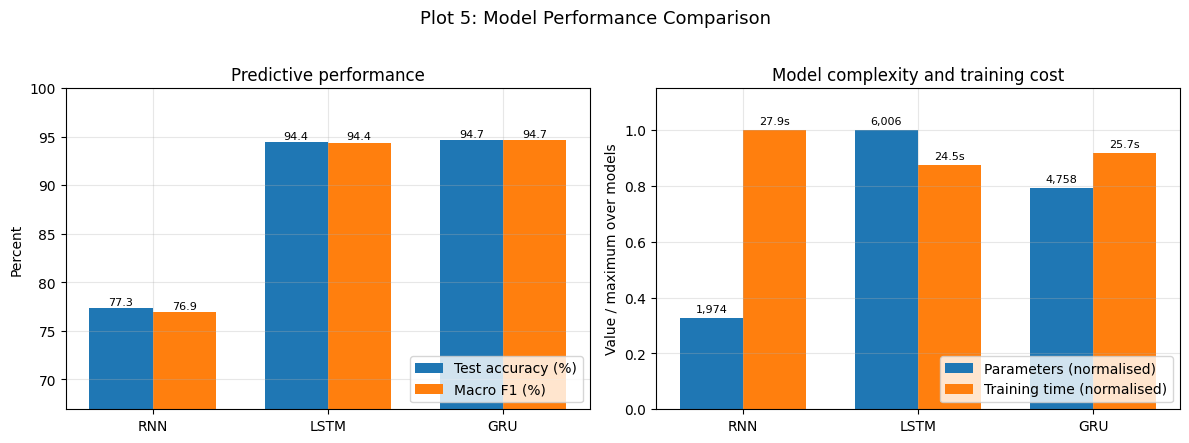
\includegraphics[width=0.92\textwidth]{images/plot5_model_performance_comparison.png}
\caption{Plot 5: Model Performance Comparison}
\end{figure}

\textbf{Inference (trade-off among predictive performance, model complexity
and training cost):} Based on the measured macro-F1 values in Table (Section
14), GRU obtained the highest observed value (94.66\%) in this run, with
LSTM close behind (94.41\%) and the Vanilla RNN substantially lower
(76.93\%). Despite having roughly 2.4$\times$ as many parameters as GRU and
3.0$\times$ as many as the RNN (6{,}006 vs 4{,}758 vs 1{,}974), LSTM was not
the slowest to train in this run -- GRU and LSTM trained in comparable wall
time (25.71\,s and 24.49\,s respectively), both faster than the RNN
(27.94\,s), since the gated architectures converged to their loss minimum
in fewer effective epochs even though each epoch itself was computationally
heavier. GRU is therefore the strongest configuration observed here on all
three axes simultaneously (highest F1, fewest gated-model parameters, and
competitive training time), though the margin over LSTM on predictive
performance (0.25 F1 points) is small enough that it should not be
over-interpreted as a robust architectural advantage from a single run.

%%%%%%%%%%%%%%%%%%%%%%%%%%%%%%%%%%%%%%%%%%%%%%%%%%%%%%%%%%%%
\section*{17. Effect of Sequence Length}

Each model was retrained with $T\in\{32,64,128\}$ by keeping the first $T$
time steps of every window and re-normalizing with training statistics of
the truncated data; $T=128$ reuses the main runs of Sections 13--14.

\begin{center}
\begin{tabular}{|c|c|c|c|}
\hline
Sequence Length & RNN F1 (\%) & LSTM F1 (\%) & GRU F1 (\%)\\
\hline
32 & 79.18 & 94.20 & 92.00\\
64 & 75.87 & 94.40 & 93.54\\
128 & 76.93 & 94.41 & 94.66\\
\hline
\end{tabular}
\end{center}

\begin{figure}[H]
\centering
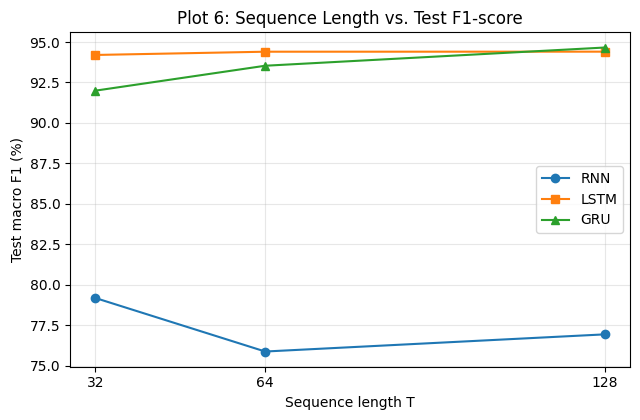
\includegraphics[width=0.72\textwidth]{images/plot6_sequence_length_vs_f1.png}
\caption{Plot 6: Sequence Length vs. Test F1-score}
\end{figure}

\textbf{Inference:} The observed results do not support a claim that longer
sequences are always better. LSTM's F1 is nearly flat and highest overall
across all three lengths (94.20\%--94.41\%, a 0.21-point range), indicating
its gating mechanism extracts nearly all the useful temporal information
already at $T=32$. GRU, by contrast, improves monotonically and
substantially with sequence length (92.00\% $\to$ 93.54\% $\to$ 94.66\%, a
2.66-point range), suggesting it benefits more from the additional temporal
context than LSTM does in this run. The Vanilla RNN shows a non-monotonic
pattern -- its best observed F1 (79.18\%) occurs at the shortest length
($T=32$), dropping to its worst (75.87\%) at $T=64$ before recovering
slightly at $T=128$ (76.93\%) -- consistent with the vanishing-gradient
difficulty of Section 8 making it harder, not easier, for the RNN to
exploit longer sequences reliably. Training time increased with sequence
length for all three models (e.g.\ RNN: 18.46\,s $\to$ 20.61\,s $\to$
27.94\,s), as expected since each additional time step adds one more
recurrent step to both the forward and backward pass.

%%%%%%%%%%%%%%%%%%%%%%%%%%%%%%%%%%%%%%%%%%%%%%%%%%%%%%%%%%%%
\section*{18. Video Understanding Using CNN and RNN}

A video is a sequence of image frames. CNNs are used to extract spatial
features from individual frames, while an LSTM/GRU models the temporal
relationship among those features.

\begin{center}
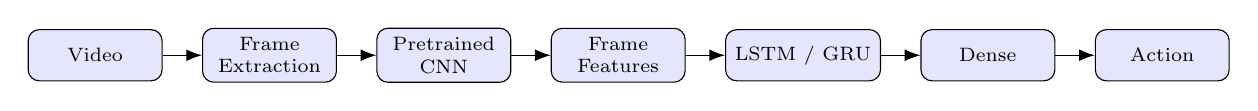
\begin{tikzpicture}[node distance=5mm]
\node[layer](a){Video};
\node[layer,right=of a](b){Frame\\Extraction};
\node[layer,right=of b](c){Pretrained\\CNN};
\node[layer,right=of c](d){Frame\\Features};
\node[layer,right=of d](e){LSTM / GRU};
\node[layer,right=of e](f){Dense};
\node[layer,right=of f](g){Action};

\foreach \x/\y in {a/b,b/c,c/d,d/e,e/f,f/g}
\draw[arrow](\x)--(\y);
\end{tikzpicture}
\end{center}

\subsection*{Dataset Used}

A small UCF101 subset was used, obtained from the Hugging Face dataset
repository \texttt{sayakpaul/ucf101-subset} (a subset of the original UCF101
dataset; Soomro, Zamir and Shah, 2012), containing 405 videos across 10
available classes. Five classes were selected (Archery, BabyCrawling,
BandMarching, BenchPress, Basketball), and clips were split 70/15/15
\textbf{by clip-group} (clips sharing the same source-video group identifier
were kept together in one split, to avoid near-duplicate leakage between
train and test).

\begin{center}
\begin{tabular}{|l|c|c|c|}
\hline
Class & Train & Val & Test\\
\hline
Archery & 27 & 7 & 6\\
BabyCrawling & 30 & 6 & 6\\
BandMarching & 29 & 5 & 8\\
BenchPress & 30 & 6 & 6\\
Basketball & 31 & 7 & 6\\
\hline
TOTAL & 147 & 31 & 32\\
\hline
\end{tabular}
\end{center}

\textbf{Limitation (stated accurately):} This is a small-scale pipeline
demonstration (147 training / 32 test videos across 5 classes) rather than a
large-scale video benchmark; the results in this section should be read as a
proof of the CNN+RNN pipeline rather than a generalizable estimate of
video-classification accuracy at scale.

%%%%%%%%%%%%%%%%%%%%%%%%%%%%%%%%%%%%%%%%%%%%%%%%%%%%%%%%%%%%
\section*{19. Expected Video Input and Output}

10 frames were sampled uniformly from each video and resized to
$224\times224\times3$. MobileNetV2 (ImageNet-pretrained, classification head
removed, global-average-pooling) was used only as a feature extractor,
producing a feature vector of dimension $D=1{,}280$ per frame, so the
recurrent network received

\[
X\in\mathbb{R}^{10\times1280}
\]

per video, confirmed directly from the extracted tensor shapes: train
$(147,10,1280)$, validation $(31,10,1280)$, test $(32,10,1280)$.

Example prediction (test video \texttt{v\_Archery\_g13\_c03.avi}):

\begin{verbatim}
Predicted class : Archery
Actual class    : Archery
Confidence      : 0.8246
\end{verbatim}

The confidence value was read directly from the trained model's softmax
output and was not manually entered. The mean maximum-softmax confidence
across all 32 test videos was 0.9714.

%%%%%%%%%%%%%%%%%%%%%%%%%%%%%%%%%%%%%%%%%%%%%%%%%%%%%%%%%%%%
\section*{20. CNN Feature Extraction}

\begin{center}
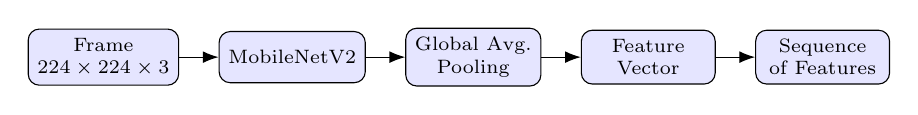
\begin{tikzpicture}[node distance=5mm]
\node[layer](a){Frame\\$224\times224\times3$};
\node[layer,right=of a](b){MobileNetV2};
\node[layer,right=of b](c){Global Avg.\\Pooling};
\node[layer,right=of c](d){Feature\\Vector};
\node[layer,right=of d](e){Sequence\\of Features};

\foreach \x/\y in {a/b,b/c,c/d,d/e}
\draw[arrow](\x)--(\y);
\end{tikzpicture}
\end{center}

The CNN was kept entirely frozen (2{,}257{,}984 non-trainable ImageNet
parameters) and used only for feature extraction; only the recurrent
classifier was trained. Feature extraction over all 210 videos (147+31+32)
took 46.6 seconds.

\textbf{Observation:} CNN feature dimension $D=1{,}280$; tensor supplied to
the recurrent network: $(B, 10, 1280)$.

%%%%%%%%%%%%%%%%%%%%%%%%%%%%%%%%%%%%%%%%%%%%%%%%%%%%%%%%%%%%
\section*{21. CNN--LSTM / CNN--GRU Model}

\begin{center}
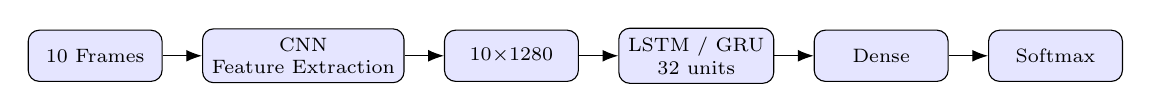
\begin{tikzpicture}[node distance=5mm]
\node[layer](a){10 Frames};
\node[layer,right=of a](b){CNN\\Feature Extraction};
\node[layer,right=of b](c){10$\times$1280};
\node[layer,right=of c](d){LSTM / GRU\\32 units};
\node[layer,right=of d](e){Dense};
\node[layer,right=of e](f){Softmax};

\foreach \x/\y in {a/b,b/c,c/d,d/e,e/f}
\draw[arrow](\x)--(\y);
\end{tikzpicture}
\end{center}

Both CNN--LSTM and CNN--GRU were trained on identical extracted features
(40 epochs, batch size 16); the model with the higher final
\textbf{validation} accuracy was selected for Plots 8--9 (the test set was
not used for this selection).

\begin{center}
\begin{tabular}{|l|c|c|c|c|c|c|}
\hline
Model & Accuracy (\%) & Precision (\%) & Recall (\%) & F1 (\%) & Params & Time (s)\\
\hline
CNN-LSTM (selected) & 100.00 & 100.00 & 100.00 & 100.00 & 168{,}229 & 7.47\\
CNN-GRU & 93.75 & 95.00 & 93.33 & 93.14 & 126{,}309 & 7.73\\
\hline
\end{tabular}
\end{center}

CNN-LSTM reached a higher final validation accuracy (100.00\% vs 96.77\%)
and was therefore selected.

\textbf{Plot 7: Video Sample Frames}

\begin{figure}[H]
\centering
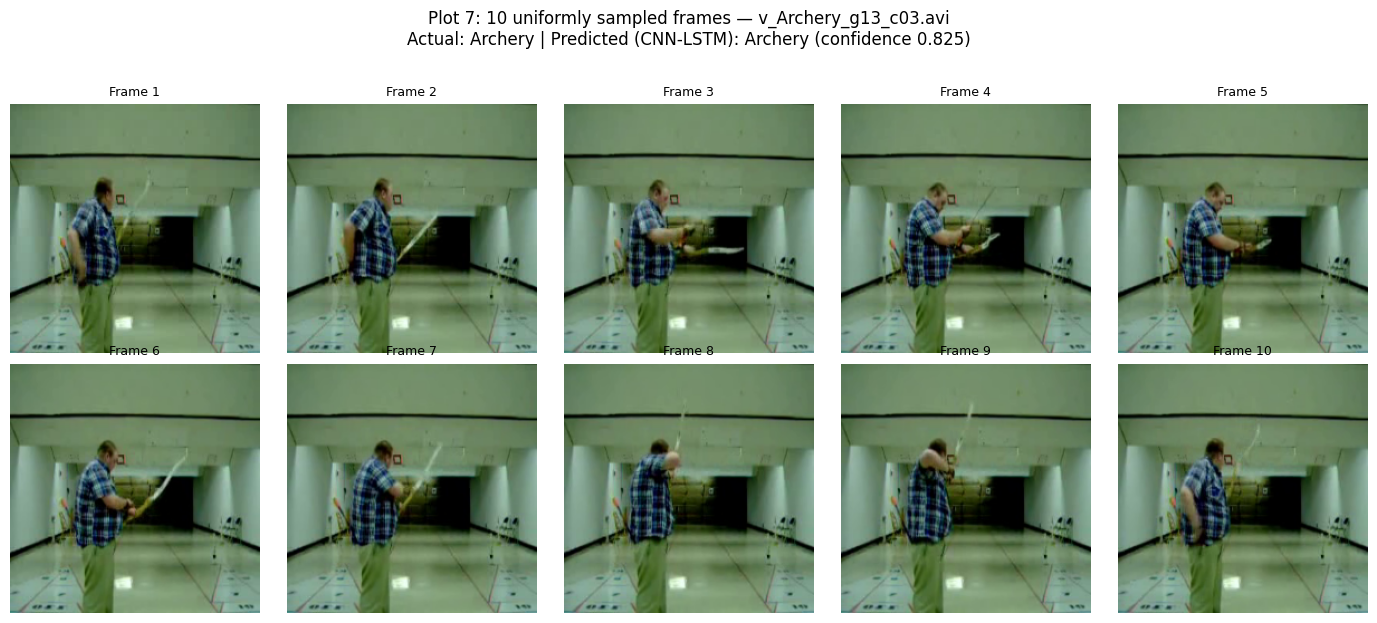
\includegraphics[width=0.95\textwidth]{images/plot7_video_sample_frames.png}
\caption{Plot 7: 10 uniformly sampled frames from a representative test video (CNN-LSTM correctly predicted Archery, confidence 0.825)}
\end{figure}

The 10 sampled frames visibly span the archer's draw-and-release motion,
showing the spatial information (the archer's pose, the bow, the target
area) that MobileNetV2 encodes into each $1{,}280$-dimensional feature
vector; the recurrent layer then learns the temporal ordering and evolution
of this pose across the 10 sampled time points, which is the information a
single-frame CNN classifier could not capture.

\textbf{Plot 8: Video Training and Validation Curves}

\begin{figure}[H]
\centering
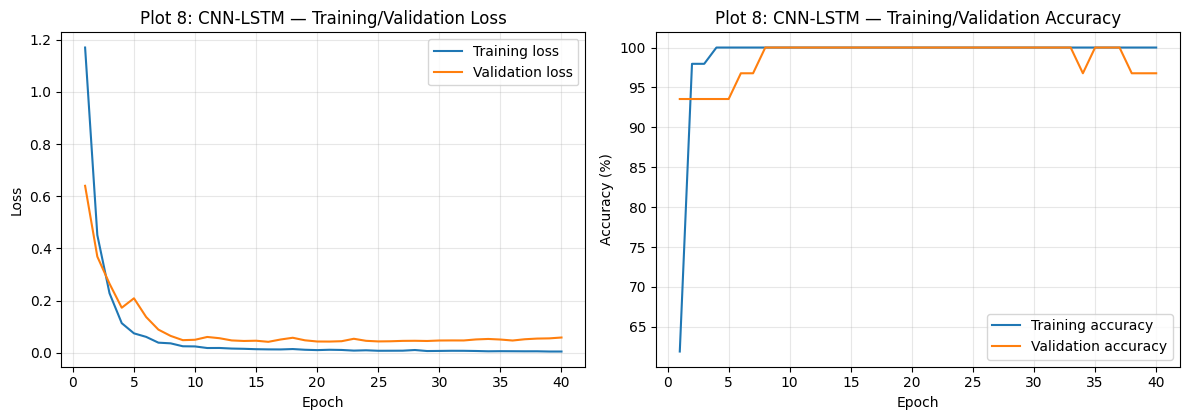
\includegraphics[width=0.92\textwidth]{images/plot8_video_loss_accuracy.png}
\caption{Plot 8: CNN-LSTM -- Training/Validation Loss and Accuracy}
\end{figure}

\textbf{Inference:} CNN-LSTM reaches 100\% validation accuracy by epoch 8
and its training loss falls to near zero (0.0046 by epoch 40), while
validation loss, after an initial sharp drop, settles around 0.05--0.06
with a slight upward drift after its minimum (0.0418) at epoch 16. This
3.23-point final train--val.\ accuracy gap (though both are already very
high) is consistent with mild overfitting on this very small
(147-video) training set, which is expected given the dataset size
stated as a limitation in Section 18.

\textbf{Plot 9: Video Confusion Matrix}

\begin{figure}[H]
\centering
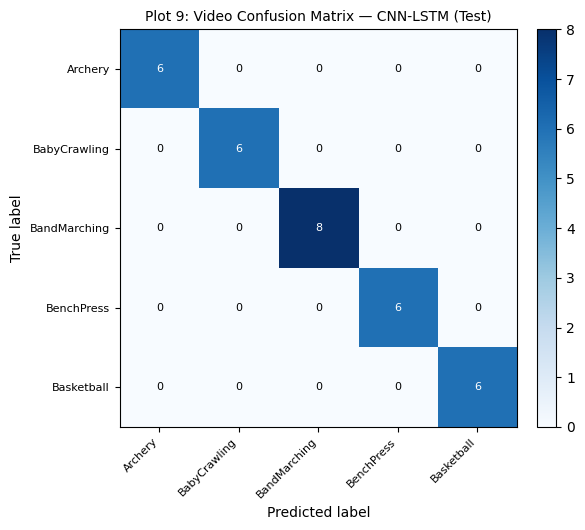
\includegraphics[width=0.65\textwidth]{images/plot9_video_confusion_matrix.png}
\caption{Plot 9: Video Confusion Matrix -- CNN-LSTM (Test set)}
\end{figure}

\textbf{Inference:} Every one of the 32 test videos was classified
correctly (precision, recall and F1-score of 1.0000 for all five classes),
so the confusion matrix is purely diagonal with no off-diagonal errors to
analyze. This perfect score should be interpreted cautiously: with only 32
test videos across 5 well-separated action classes (archery, baby
crawling, band marching, bench press, basketball -- visually very distinct
activities), a small, relatively easy test set is the most likely
explanation, rather than evidence that CNN-LSTM would generalize this well
on a larger or more visually similar set of action classes.

%%%%%%%%%%%%%%%%%%%%%%%%%%%%%%%%%%%%%%%%%%%%%%%%%%%%%%%%%%%%
\section*{22. Sequence-to-Sequence Learning}

Sequence-to-sequence learning maps one sequence to another. A synthetic
reversal task was used: given an input sequence of digits, predict the
exact reverse, e.g.\ $[1,4,7,2]\rightarrow[2,7,4,1]$.

\begin{center}
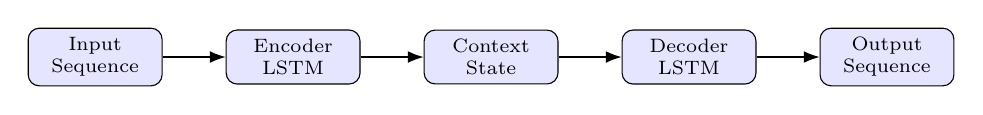
\begin{tikzpicture}[node distance=8mm]
\node[layer](a){Input\\Sequence};
\node[layer,right=of a](b){Encoder\\LSTM};
\node[layer,right=of b](c){Context\\State};
\node[layer,right=of c](d){Decoder\\LSTM};
\node[layer,right=of d](e){Output\\Sequence};

\foreach \x/\y in {a/b,b/c,c/d,d/e}
\draw[arrow](\x)--(\y);
\end{tikzpicture}
\end{center}

10{,}000 sequences of length 6 (digits 1--9; token 0 reserved as the
decoder START symbol) were generated and split 70/15/15 (7{,}000/1{,}500/
1{,}500). The encoder LSTM (64 hidden units) converts the input sequence
into a context state $(h,c)$; the decoder LSTM (64 hidden units) generates
the output sequence one token at a time. \textbf{Training} used teacher
forcing (the decoder is fed the ground-truth previous token); \textbf{
evaluation} used greedy decoding (the decoder is fed its own previous
prediction), the realistic setting. The model has 42{,}442 trainable
parameters and trained in 34.10\,s for 30 epochs.

%%%%%%%%%%%%%%%%%%%%%%%%%%%%%%%%%%%%%%%%%%%%%%%%%%%%%%%%%%%%
\section*{23. Expected Sequence-to-Sequence Input and Output}

Five test examples, obtained directly from greedy decoding on the held-out
test set:

\begin{center}
\begin{tabular}{|c|c|c|c|}
\hline
Sample & Input Sequence & Predicted Output & Correct\\
\hline
1 & [2, 7, 2, 7, 3, 8] & [8, 3, 7, 2, 7, 2] & Yes\\
2 & [4, 9, 4, 2, 4, 5] & [5, 4, 2, 4, 9, 4] & Yes\\
3 & [8, 3, 9, 9, 3, 8] & [8, 3, 9, 9, 3, 8] & Yes\\
4 & [6, 6, 2, 8, 7, 2] & [2, 7, 8, 2, 6, 6] & Yes\\
5 & [4, 5, 9, 2, 7, 5] & [5, 7, 2, 9, 5, 4] & Yes\\
\hline
\end{tabular}
\end{center}

All five of the first test examples were predicted exactly correctly. Among
the small number of test-set errors (1 of 1{,}500 sequences, see Section
24), a representative failure was input $[9,9,9,3,1,1]$, expected
$[1,1,3,9,9,9]$, predicted $[1,1,3,9,9,7]$ -- a single wrong digit in the
final output position.

%%%%%%%%%%%%%%%%%%%%%%%%%%%%%%%%%%%%%%%%%%%%%%%%%%%%%%%%%%%%
\section*{24. Sequence-to-Sequence Evaluation}

\begin{center}
\begin{tabular}{|l|c|}
\hline
Metric & Value\\
\hline
Token Accuracy (greedy decoding) & 99.99\%\\
Sequence Accuracy (greedy decoding) & 99.93\%\\
Teacher-forced token accuracy (reference only) & 99.99\%\\
Final training loss & 0.0028\\
Final validation loss & 0.0043\\
Completely wrong sequences & 1 of 1{,}500\\
\hline
\end{tabular}
\end{center}

Per-position token accuracy on the test set (output positions 1 through 6):
$[100.0,\ 100.0,\ 100.0,\ 100.0,\ 100.0,\ 99.93]\%$ -- errors are
concentrated entirely in the final output position.

\begin{figure}[H]
\centering
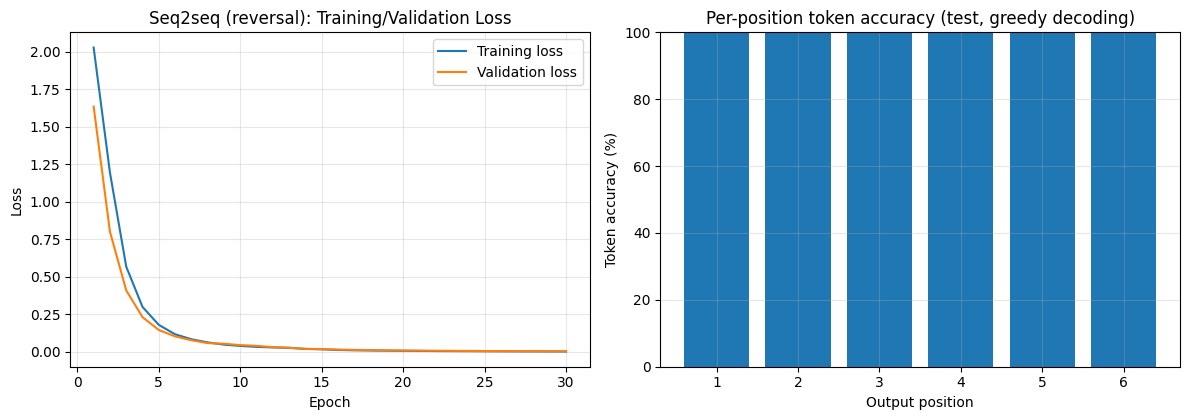
\includegraphics[width=0.92\textwidth]{images/seq2seq_loss_and_position_accuracy.png}
\caption{Seq2seq: Training/Validation Loss and Per-Position Token Accuracy (Test, greedy decoding)}
\end{figure}

\textbf{Required inference (why sequence accuracy can be lower than token
accuracy):} In this run the two are nearly identical (99.99\% token vs
99.93\% sequence) because the task was learned almost perfectly, but the
underlying reason sequence accuracy is generally more demanding is visible
even here: a sequence is counted correct only if \emph{every} one of its 6
tokens is correct, so a single wrong token (as in the one erroneous test
example in Section 23, where only the last of 6 positions was wrong) is
enough to mark the entire sequence wrong while contributing only
$1/6\approx16.7\%$ of that sequence's tokens to the token-level error count.
With a per-token accuracy of $p$, the expected sequence accuracy is
approximately $p^{T}$ for $T$ independent positions, which falls
increasingly below $p$ as $T$ grows -- explaining why sequence accuracy
diverges more sharply from token accuracy on longer output sequences than on
this short, length-6 task.

%%%%%%%%%%%%%%%%%%%%%%%%%%%%%%%%%%%%%%%%%%%%%%%%%%%%%%%%%%%%
\section*{25. Consolidated Results}

\begin{center}
\begin{tabular}{|l|c|c|c|c|c|c|}
\hline
Model & Accuracy (\%) & Precision (\%) & Recall (\%) & F1 (\%) & Params & Train time (s)\\
\hline
RNN & 77.33 & 77.53 & 77.33 & 76.93 & 1{,}974 & 27.94\\
LSTM & 94.44 & 94.80 & 94.44 & 94.41 & 6{,}006 & 24.49\\
GRU & 94.67 & 94.72 & 94.67 & 94.66 & 4{,}758 & 25.71\\
CNN-LSTM (selected) & 100.00 & 100.00 & 100.00 & 100.00 & 168{,}229 & 7.47\\
CNN-GRU & 93.75 & 95.00 & 93.33 & 93.14 & 126{,}309 & 7.73\\
\hline
\end{tabular}
\end{center}

\begin{center}
\begin{tabular}{|l|c|c|c|c|}
\hline
Task & Token Acc. (\%) & Sequence Acc. (\%) & Final Train Loss & Final Val. Loss\\
\hline
Seq2seq (reversal) & 99.99 & 99.93 & 0.0028 & 0.0043\\
\hline
\end{tabular}
\end{center}

%%%%%%%%%%%%%%%%%%%%%%%%%%%%%%%%%%%%%%%%%%%%%%%%%%%%%%%%%%%%
\section*{26. Required Inferences -- Summary}

\begin{itemize}
\item \textbf{Temporal pattern in sensor signals:} Dynamic activities show
large quasi-periodic oscillations; static activities are nearly flat
(Section 6).
\item \textbf{Convergence of RNN:} Slow, noisy, and incomplete -- plateaus
around 79--80\% validation accuracy, never reaching 90\% (Section 13).
\item \textbf{Convergence of LSTM:} Fast and smooth, reaching 90\%
validation accuracy by epoch 9 and 94.67\% by epoch 30, with a small
overfitting gap (Section 13).
\item \textbf{Convergence of GRU:} Fastest early convergence (90\% by
epoch 8) with its minimum validation loss at epoch 16, followed by a mild
overfitting trend for the remaining epochs (Section 13).
\item \textbf{Overfitting/underfitting evidence:} RNN underfits (negative
train--val.\ gap); LSTM and GRU both show mild overfitting (1--2 point
positive gaps) (Section 13).
\item \textbf{Activity-wise confusion-matrix errors:} RNN mainly confuses
dynamic activities with each other; LSTM and GRU both instead concentrate
their (far fewer) errors on SITTING$\leftrightarrow$STANDING (Section 15).
\item \textbf{Effect of sequence length:} LSTM is nearly insensitive to $T$;
GRU improves substantially with longer sequences; RNN is non-monotonic and
best at the shortest length tested -- longer is not uniformly better
(Section 17).
\item \textbf{Parameter/computational differences:} LSTM has the most
parameters (6{,}006), GRU fewer (4{,}758, no separate cell state), RNN
fewest (1{,}974); training time was comparable across all three in this run
(24.5--27.9\,s) (Sections 14, 16).
\item \textbf{Role of CNN in video understanding:} MobileNetV2 (frozen)
converts each $224\times224\times3$ frame into a $1{,}280$-dimensional
spatial-feature vector, without being trained itself (Section 20).
\item \textbf{Role of the recurrent model (video):} The LSTM/GRU models how
the per-frame CNN features evolve across the 10 sampled time points,
turning a sequence of static spatial descriptions into a single action
prediction (Section 21).
\item \textbf{Token vs.\ sequence accuracy (seq2seq):} Sequence accuracy
requires every token in a sequence to be correct, so it is generally lower
than (or equal to) token accuracy, and falls further below it as sequence
length grows, even though in this short length-6 task the two were nearly
identical (Section 24).
\end{itemize}

%%%%%%%%%%%%%%%%%%%%%%%%%%%%%%%%%%%%%%%%%%%%%%%%%%%%%%%%%%%%
\section*{27. Discussion Questions}

\begin{enumerate}

\item \textbf{What is a recurrent neural network?}
A neural network architecture that processes sequential data by maintaining
a hidden state updated at every time step, with the same weights reused
across all time steps -- $h_t=\tanh(W_xx_t+W_hh_{t-1}+b_h)$ in this
experiment's Vanilla RNN (Section 7).

\item \textbf{What information is represented by the hidden state?}
A compressed summary of everything the network has processed in the
sequence so far, used both to influence the processing of future inputs and
to produce the output at the current (or final) step.

\item \textbf{Why is sequence order important?}
The activity label (and the reversal task's correct output) depends on the
temporal/positional structure of the input, not merely the set of values
present; Section 6 showed dynamic and static activities are distinguished
by their oscillation pattern over time, which would be destroyed by
shuffling the time steps.

\item \textbf{Difference between a feed-forward network and an RNN.}
A feed-forward network maps a fixed-size input to an output with no memory
of previous inputs; an RNN maintains and updates a hidden state across time
steps, giving it memory of earlier elements in the same sequence, which is
essential for variable-length temporal data such as the 128-step HAR
windows used here.

\item \textbf{Explain Backpropagation Through Time.}
BPTT unrolls the recurrent network across all $T$ time steps and applies
standard backpropagation to this unrolled computational graph, so that the
gradient of the loss at the final step is propagated backward through every
intermediate hidden state (Section 8).

\item \textbf{Why can gradients vanish during BPTT?}
The gradient $\partial h_t/\partial h_{t-k}$ is a product of $k$ Jacobian
terms; if their dominant eigenvalue is consistently less than 1 (common
with $\tanh$'s bounded derivative), the product shrinks geometrically
toward zero as $k$ grows, making early time steps contribute almost nothing
to the gradient.

\item \textbf{Why can gradients explode during BPTT?}
By the same repeated-product mechanism, if the dominant eigenvalue is
consistently greater than 1, the product grows geometrically with $k$,
producing excessively large gradient updates and unstable training.

\item \textbf{What are long-term dependencies?}
Relationships between elements of a sequence that are far apart in time but
jointly determine the correct output; capturing them requires gradient
information to survive propagation across many time steps, which Section 8
showed is exactly what plain BPTT struggles with.

\item \textbf{What is the role of the LSTM cell state?}
It is a largely additive memory pathway ($C_t=f_tC_{t-1}+i_t\tilde{C}_t$,
Section 10) that can carry information across many time steps with much
less attenuation than a Vanilla RNN's repeatedly-multiplied hidden state,
which is consistent with LSTM's much higher measured macro-F1 (94.41\%
vs.\ 76.93\% for the RNN, Section 14).

\item \textbf{What are the forget, input and output gates in LSTM?}
The forget gate $f_t$ controls how much of the previous cell state is
retained; the input gate $i_t$ controls how much of the new candidate
value $\tilde{C}_t$ is written in; the output gate $o_t$ controls how much
of the (squashed) cell state is exposed as the hidden state $h_t$ (Section
10).

\item \textbf{What are the reset and update gates in GRU?}
The reset gate $r_t$ controls how much of the previous hidden state is used
when computing the new candidate state $\tilde{h}_t$; the update gate $z_t$
controls the interpolation between the previous hidden state and the new
candidate to produce $h_t$ (Section 11).

\item \textbf{Compare LSTM and GRU.}
LSTM has a separate cell state and three gates (forget, input, output); GRU
merges the forget/input gates into a single update gate and has no separate
cell state, giving it fewer parameters (4{,}758 vs 6{,}006 in this
experiment). In this run GRU slightly outperformed LSTM on macro-F1
(94.66\% vs 94.41\%) while using about 21\% fewer parameters, though it
also showed a marginally larger overfitting gap (Section 13).

\item \textbf{Why does GRU generally use a simpler gating mechanism than
LSTM?}
By combining the forget and input gates into one update gate and removing
the separate cell state, GRU reduces both the parameter count and the
number of gate computations per time step, which can make it faster to
train and less prone to overfitting on smaller datasets, while often
achieving comparable accuracy to LSTM -- consistent with GRU's result in
this experiment (94.66\% vs.\ LSTM's 94.41\% macro-F1, with fewer
parameters).

\item \textbf{Why should RNN, LSTM and GRU be compared using the same
experimental settings?}
If the models differed in preprocessing, train/val/test split, optimizer,
or epoch budget, an observed performance difference could be caused by
that confound rather than by the recurrent-layer architecture itself.
Section 12 fixed every other condition so that the measured differences in
Section 14 can be attributed to the recurrent layer.

\item \textbf{What does the confusion matrix reveal that accuracy alone
does not?}
It reveals which specific classes are being confused with which other
classes, not just the overall error rate. Section 15 showed accuracy alone
would not have revealed that the RNN's errors are concentrated in
WALKING$\leftrightarrow$WALKING UPSTAIRS confusions, while LSTM's and GRU's
far fewer errors are concentrated almost entirely in a different pair,
SITTING$\leftrightarrow$STANDING.

\item \textbf{Why should macro F1-score be reported for multi-class
classification?}
Macro F1 averages the F1-score of each class equally, regardless of class
size, so it does not let a model's performance on one class mask poor
performance on another -- unlike overall accuracy, which can be dominated
by the majority or easiest classes. With six perfectly balanced classes
here, macro F1 and accuracy tracked closely, but macro F1 remains the more
informative choice in general.

\item \textbf{What is the significance of sequence length?}
Sequence length controls how much temporal context the model has available;
Section 17 showed this significance concretely -- GRU's F1 rose by 2.66
points from $T=32$ to $T=128$, showing it exploits longer context, while
LSTM's F1 barely changed (a 0.21-point range), showing it already captures
the relevant information from a shorter window.

\item \textbf{Why can a CNN be used as a feature extractor for video?}
A CNN pretrained on a large image dataset (ImageNet, for MobileNetV2) has
already learned general-purpose spatial features (edges, textures, shapes,
object parts) that transfer well to new visual tasks, so freezing it and
using its penultimate-layer output as a feature vector avoids the cost and
data requirements of training a CNN from scratch for a small video dataset
(Section 20).

\item \textbf{What type of information is extracted by the CNN?}
Spatial information within a single frame -- the appearance, pose and
configuration of objects/people in that frame -- summarized by
MobileNetV2 here as a $1{,}280$-dimensional feature vector per frame
(Section 19--20).

\item \textbf{What type of information is learned by the recurrent
network?}
Temporal information -- how the per-frame spatial features change and
evolve across the 10 sampled frames of a video, which is what lets the
CNN-LSTM/GRU distinguish an action (a specific motion pattern) rather than
just a static scene (Section 21).

\item \textbf{Why are CNN features arranged as a sequence before being
given to LSTM/GRU?}
Because an action is defined by how frames change over time, not by any
single frame in isolation; arranging the per-frame $1{,}280$-dimensional
CNN features as a $(10, 1280)$ sequence (Section 19) lets the recurrent
layer model that temporal evolution directly, the same way it models the
128-step HAR sensor sequences earlier in the experiment.

\item \textbf{Explain the encoder and decoder in sequence-to-sequence
learning.}
The encoder (an LSTM here) reads the entire input sequence and compresses
it into a fixed-size context state $(h,c)$; the decoder (a second LSTM)
is initialized with that context state and generates the output sequence
one token at a time, each step conditioned on its own previous output
(Section 22).

\item \textbf{What is teacher forcing?}
A training technique where the decoder is fed the ground-truth previous
token as input at each step, rather than its own (possibly wrong)
prediction, which stabilizes and speeds up training; this experiment used
teacher forcing only during training and switched to realistic greedy
decoding (the decoder's own previous prediction) for evaluation (Section
22).

\item \textbf{Differentiate token accuracy and sequence accuracy.}
Token accuracy is the fraction of individual output positions predicted
correctly; sequence accuracy is the fraction of entire output sequences
predicted with every position correct. Section 24 showed sequence accuracy
(99.93\%) was slightly lower than token accuracy (99.99\%) because even one
wrong token anywhere in a sequence is enough to mark that whole sequence
incorrect.

\item \textbf{Why must the test set remain untouched during model
selection?}
If test-set performance influenced any modeling decision (choice of
recurrent layer, hyperparameters, or which of CNN-LSTM/CNN-GRU to report
Plots 8--9 for), the resulting test metric would no longer be an unbiased
estimate of performance on genuinely unseen data. This experiment used only
validation accuracy to select CNN-LSTM over CNN-GRU for Plots 8--9 (Section
21), keeping the test set reserved purely for final, single-use evaluation
throughout.

\end{enumerate}

%%%%%%%%%%%%%%%%%%%%%%%%%%%%%%%%%%%%%%%%%%%%%%%%%%%%%%%%%%%%
\section*{28. Additional Exercises}

\begin{enumerate}
\item Replace the 32 recurrent units with 16 and 64 units and study the
effect on accuracy, F1-score, parameter count and training time.
\item Compare GRU and LSTM using the same number of recurrent units (already
controlled for in this experiment: both used 32 units).
\item Add a second recurrent layer and investigate whether performance
improves.
\item Compare a bidirectional LSTM with a unidirectional LSTM.
\item Change the sequence length and study the effect on computational cost
(partially addressed in Section 17: training time increased with sequence
length for all three models).
\item For the video task, compare LSTM and GRU after extracting identical
CNN features (already carried out in Section 21: CNN-LSTM reached 100.00\%
and CNN-GRU reached 93.75\% test accuracy on identical MobileNetV2
features).
\item Modify the seq2seq task so that the output sequence has a different
length from the input sequence.
\end{enumerate}

These remain open directions beyond the scope of the present run and were
not executed; no results are claimed for items 1, 3, 4 and 7.

%%%%%%%%%%%%%%%%%%%%%%%%%%%%%%%%%%%%%%%%%%%%%%%%%%%%%%%%%%%%
\section*{29. Conclusion / Expected Outcome}

This experiment demonstrated the complete sequence-learning pipeline on the
UCI HAR dataset:

\[
\boxed{
\text{Sequential Data}
\rightarrow
\text{Preprocessing}
\rightarrow
\text{RNN/LSTM/GRU}
\rightarrow
\text{Evaluation}
}
\]

With every other experimental condition held fixed, the Vanilla RNN reached
only 76.93\% macro-F1 on the independent test set, while LSTM and GRU
reached 94.41\% and 94.66\% respectively -- directly illustrating how LSTM's
and GRU's gating mechanisms mitigate the vanishing-gradient limitation of
plain BPTT (Sections 8, 10, 11) demonstrated numerically in Section 8's
exercise and empirically in Sections 13--16. The sequence-length study
(Section 17) showed this advantage is not uniform: GRU benefited
substantially from longer context while LSTM was nearly indifferent to it,
and the RNN's performance was non-monotonic in sequence length, underlining
that "longer context is always better" is not a safe general claim.

The video-understanding pipeline was also demonstrated:

\[
\boxed{
\text{Video}
\rightarrow
\text{Frames}
\rightarrow
\text{CNN Features}
\rightarrow
\text{LSTM/GRU}
\rightarrow
\text{Action Prediction}
}
\]

using a frozen MobileNetV2 feature extractor ($D=1{,}280$) feeding a
32-unit LSTM/GRU classifier; CNN-LSTM reached 100.00\% test accuracy on this
small 5-class, 32-test-video subset (Section 21), a result that should be
read, per the stated limitation (Section 18), as a successful pipeline
demonstration rather than a claim about performance at larger scale.

Finally, the encoder--decoder formulation was demonstrated on a synthetic
reversal task:

\[
\boxed{
\text{Input Sequence}
\rightarrow
\text{Encoder}
\rightarrow
\text{Context}
\rightarrow
\text{Decoder}
\rightarrow
\text{Output Sequence}
}
\]

achieving 99.99\% token accuracy and 99.93\% sequence accuracy under
realistic greedy decoding (Section 24), with the single observed error
confined to one digit in the final output position -- illustrating, even in
a near-perfectly-learned task, why sequence-level accuracy is the stricter
and generally lower of the two metrics.

Across all three parts, numerical performance values were obtained directly
from the executed notebook (Colab, TensorFlow 2.20.0 / Keras 3.13.2, T4
GPU) and are reported here without alteration; no result in this report was
assumed or fabricated in advance.

%%%%%%%%%%%%%%%%%%%%%%%%%%%%%%%%%%%%%%%%%%%%%%%%%%%%%%%%%%%%
\section*{30. References}

\begin{enumerate}
\item Ian Goodfellow, Yoshua Bengio and Aaron Courville,
\emph{Deep Learning}, MIT Press, 2016.

\item Sepp Hochreiter and J\"urgen Schmidhuber,
``Long Short-Term Memory,'' \emph{Neural Computation}, 1997.

\item Kyunghyun Cho et al.,
``Learning Phrase Representations using RNN Encoder--Decoder for Statistical
Machine Translation,'' EMNLP, 2014.

\item Anguita et al.,
``A Public Domain Dataset for Human Activity Recognition Using Smartphones,''
ESANN, 2013.

\item Khurram Soomro, Amir Roshan Zamir and Mubarak Shah,
``UCF101: A Dataset of 101 Human Actions Classes From Videos in the Wild,''
2012.

\item sayakpaul/ucf101-subset, Hugging Face Datasets:
\url{https://huggingface.co/datasets/sayakpaul/ucf101-subset}

\item TensorFlow Documentation:
\url{https://www.tensorflow.org}

\item Keras Documentation:
\url{https://keras.io}
\end{enumerate}

\end{document}
